\section{Physical View}
\label{sec_deployment}


\subsection{Overview}

The purpose of the physical view is to describe the mapping of the software onto the hardware and to illustrate the software's distributed aspects.


\subsection{Stakeholders}

\textbf{\textit{Developers, Testers, Users}}

\textit{A description of all stakeholders is contained in Section \ref{sec:stakeholders}.}


\subsection{General Application}

In a typical application (see Figure \ref{fig:deployment_client_server}) a general purpose version of the library will be built and incorporated within third party applications as either a static or a shared library. This deployment scenario does not require the library to be built with any particular emphasis on compiled size, memory footprint or processor utilisation.

\begin{figure}[H]
\centering
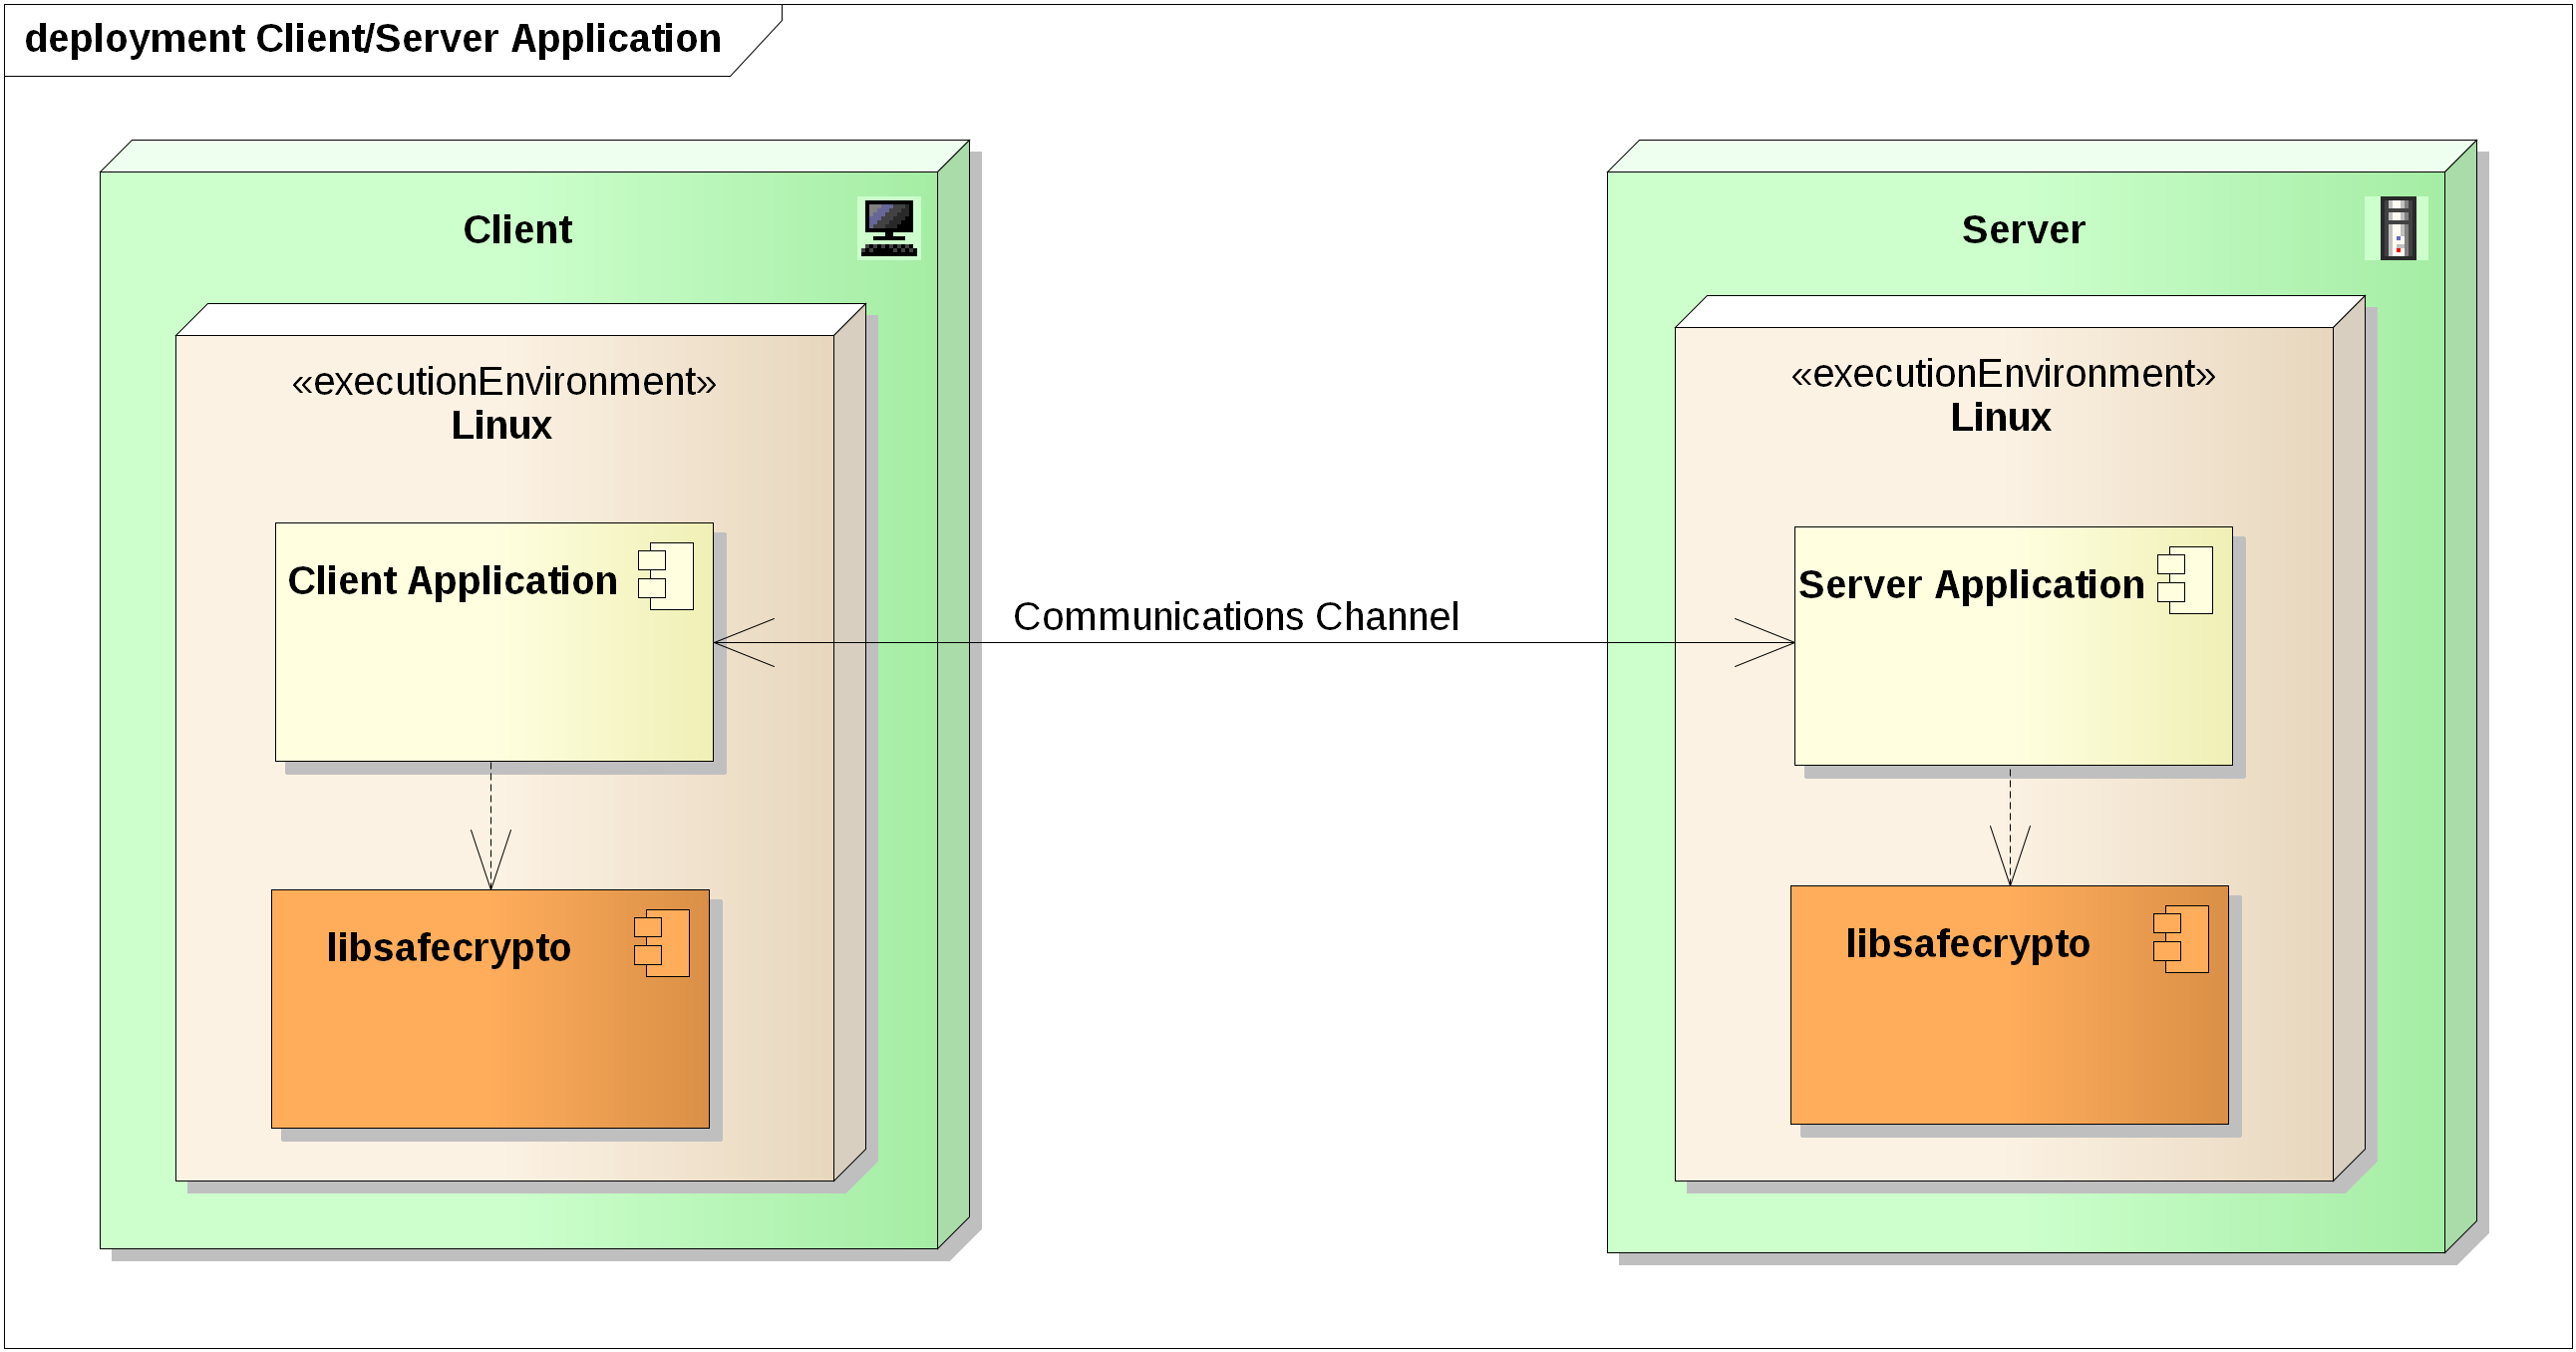
\includegraphics[width=0.9\textwidth]{simple_deployment_client_server.png}
\caption{Deployment diagram of a typical client/server application}
\label{fig:deployment_client_server}
\end{figure}

\subsection{Constrained Application}

A typical build will rely upon the build system to create a compiled version of the library that takes advantage of the processor capabilities of the system, such as SIMD instructions or 64-bit word size. However, in some deployment scenarios the device will be constrained to some extent. Under these circumstances it is possible to build the library to vary the executable size, memory footprint and processor utilisation to varying degrees in order to achieve acceptable performance on the target hardware platform.

The SAFEcrypto library will provide compile-time switches that vary the processor, memory and storage requirements of the library to more optimally suit the target platform. In addition, the target application can be targetted to provide a general purpose, client-only or server-only build of the library.

In an embedded device (see Figure \ref{fig:deployment_constrained}) the library can be built to operate as a client only, excluding the software features and associated resources that are required for server operation. Additionally, the memory resources can be constrained to reduce RAM or ROM use as necessary depending upon the physical capabilities of the target hardware. In contrast to an embedded device a high end server has abundant processor, RAM and storage capabilities that the SAFEcrypto library can exploit in a targeted build. In addition, a server application may or may not require many features necessary for a client application.

\begin{figure}[ht]
\centering
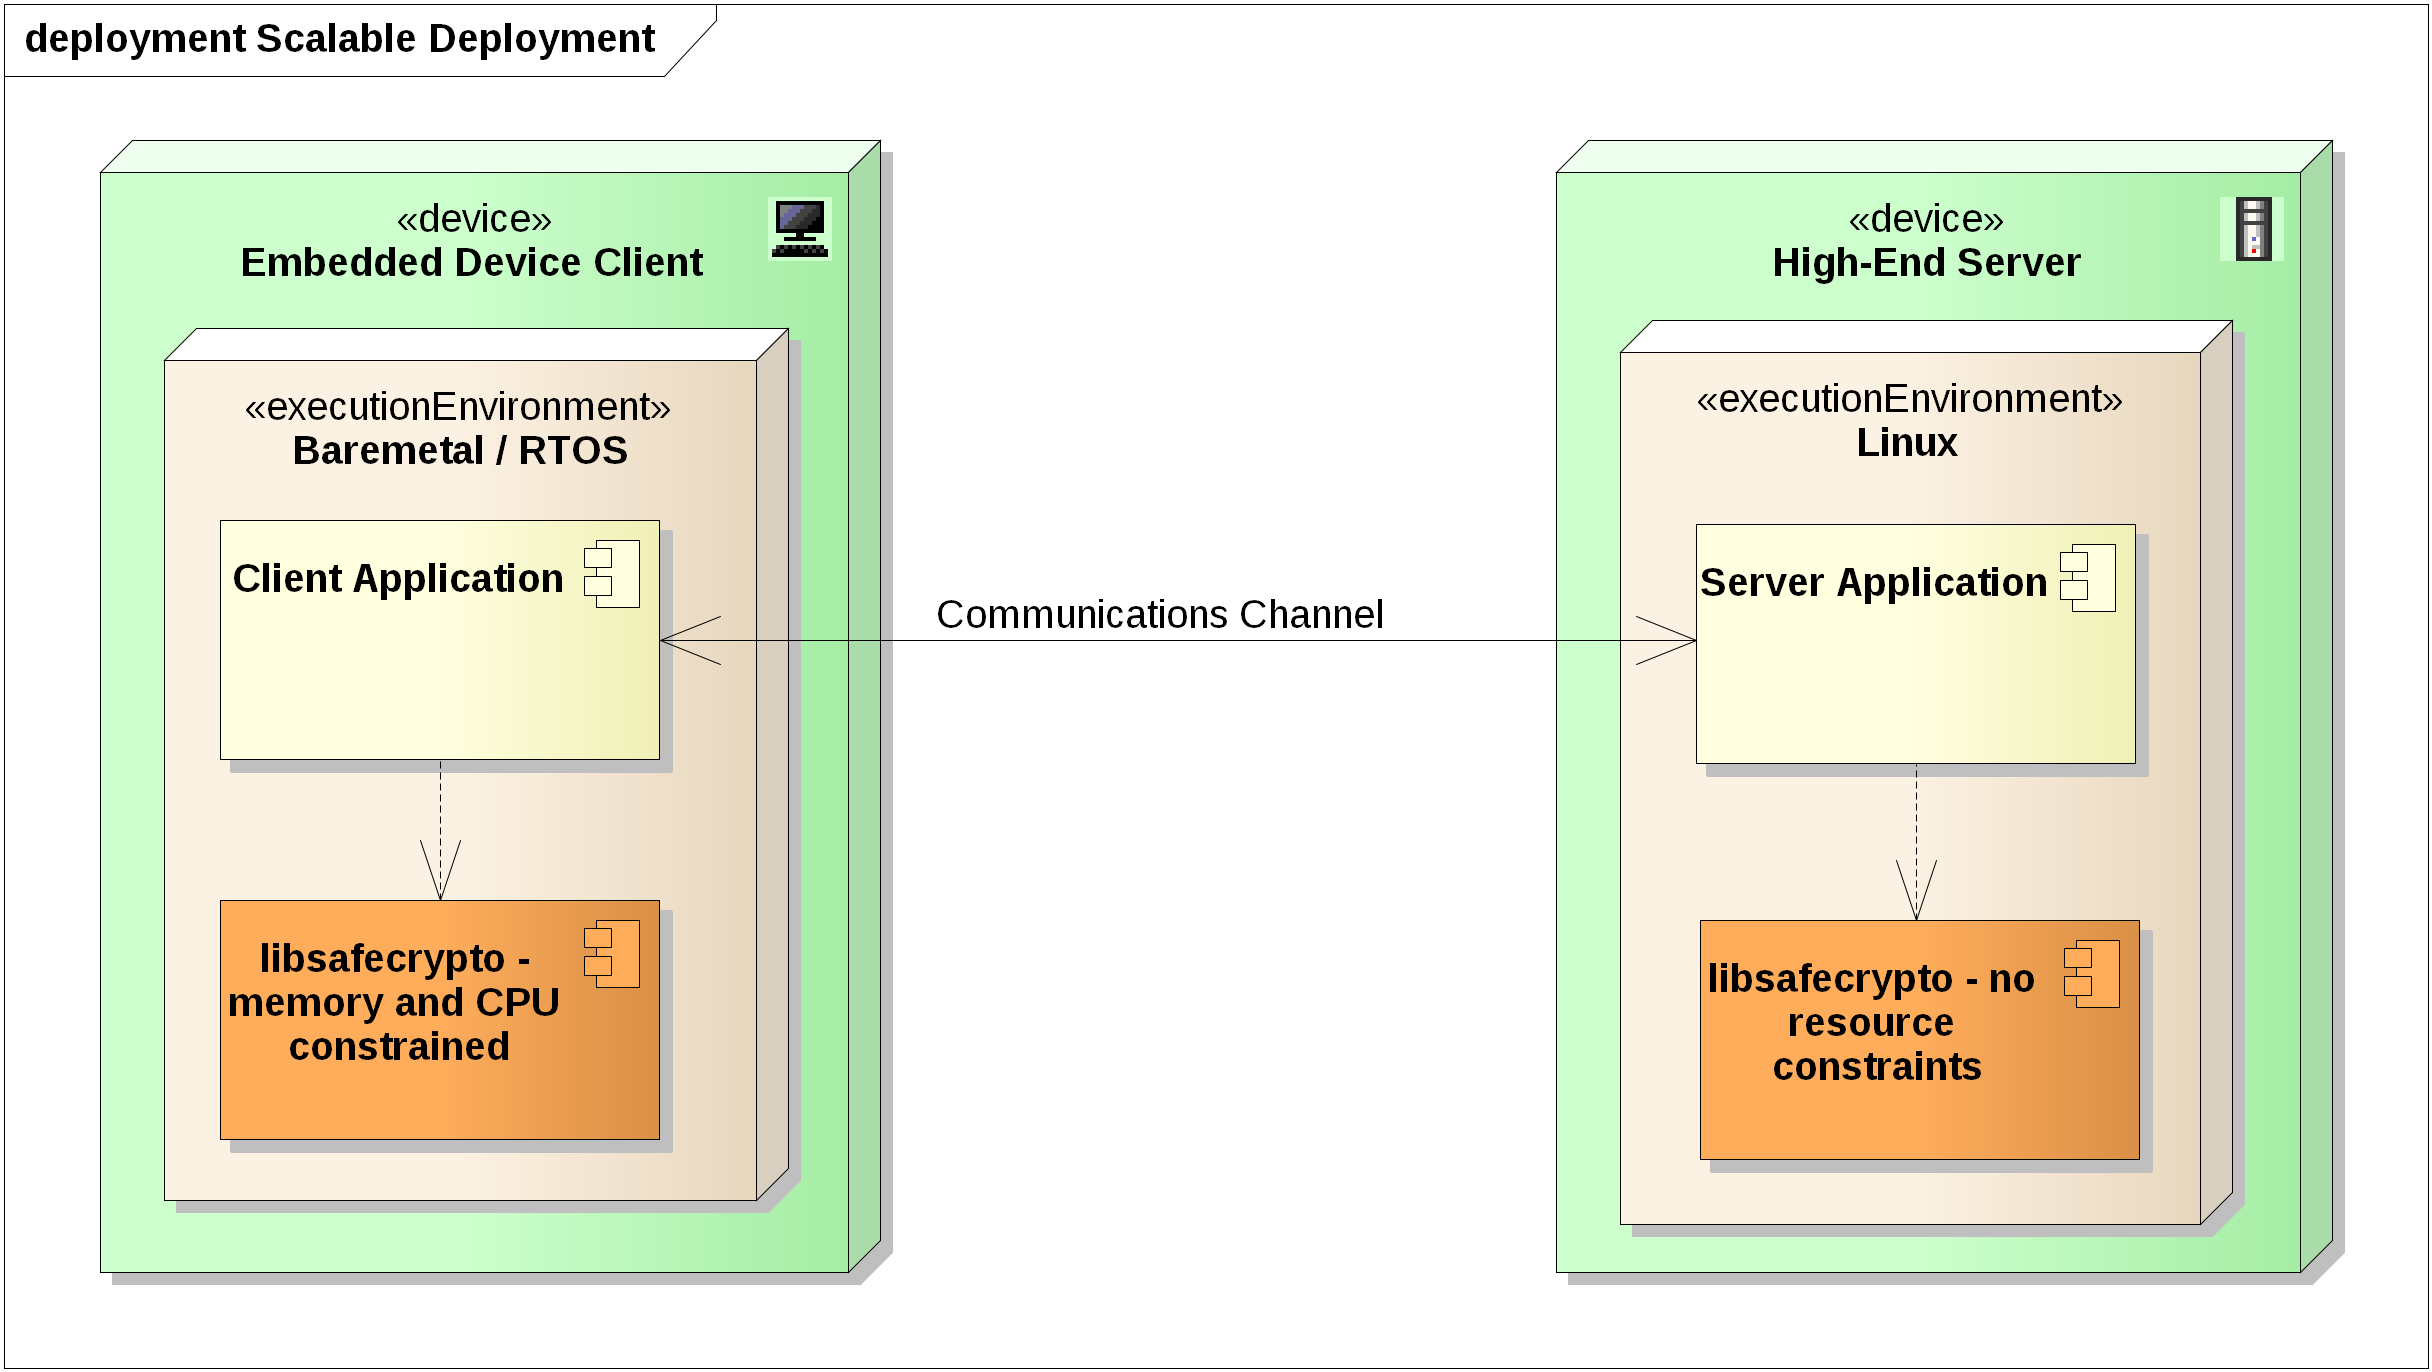
\includegraphics[width=0.9\textwidth]{scaled_deployment_client_server.png}
\caption{Deployment diagram of a high-bandwidth server application}
\label{fig:deployment_constrained}
\end{figure}

